\documentclass[11pt]{article}
\usepackage[margin=1in]{geometry}
\usepackage[T1]{fontenc}
\usepackage[utf8]{inputenc}
\usepackage{lmodern}
\usepackage{amsmath,amssymb,mathtools}
\usepackage{physics}
\usepackage{booktabs}
\usepackage{array}
\usepackage{enumitem}
\usepackage[table]{xcolor}
\usepackage{hyperref}
\usepackage{microtype}
\usepackage{parskip}
\usepackage{titlesec}
\usepackage{tabularx}
\usepackage{longtable}
\usepackage{tikz}
\usetikzlibrary{arrows.meta,positioning,shapes.geometric,fit,backgrounds}
\titleformat{\section}{\large\bfseries}{}{0em}{}
\titleformat{\subsection}{\normalsize\bfseries}{}{0em}{}
\hypersetup{colorlinks=true,linkcolor=blue,urlcolor=blue}
\newcommand{\kb}{k_\mathrm{B}}
\newcommand{\taueff}{\tau_\mathrm{eff}}
\newcolumntype{Y}{>{\raggedright\arraybackslash}X}
\begin{document}

\title{Module 0: Project Overview and Phase Map \\ From Radiation-Induced Defects to Device Degradation in Silicon}
\author{}
\date{}
\maketitle

\section{Purpose of this overview}
This document is the map of the whole project. The later modules go deep into the physics, derivations, and assumptions inside each phase. This overview answers a simpler question first: \emph{how do all of the pieces fit together?}

The project tells one continuous story:
\begin{center}
incident radiation $\to$ transport in silicon $\to$ displacement-like events $\to$ defect population $\to$ semiconductor property changes $\to$ device degradation $\to$ cryogenic persistence and slower recovery.
\end{center}

A useful analogy is a winter road after a storm. The storm itself is the radiation field. Tire tracks and impacts in the snow are the transport and collision history. Cracks and potholes are the defects. The way the road drives afterward is the device-level degradation. If the temperature later drops far below freezing, the road damage can become locked in and much slower to heal. That final low-temperature behavior is the cryogenic extension of this project.

\section{The five-module structure}
The project is organized into five modules.

\begin{center}
\rowcolors{2}{gray!8}{white}
\begin{tabularx}{\textwidth}{>{\bfseries}p{0.10\textwidth} >{\bfseries}p{0.27\textwidth} Y Y}
\toprule
Phase & Module title & Main physics question & Main output \\
\midrule
0 & Project overview and phase map & How do all parts connect into one causal chain? & Global roadmap and workflow \\
1 & Geant4 transport and damage proxies & What happens when radiation enters silicon? & Depth deposition, event deposition, recoil-like proxies \\
2 & Defect generation and solid-state interpretation & How do interaction histories become defects and traps? & Defect-density model and interpretation of lattice damage \\
3 & Room-temperature device degradation & How do defects alter lifetime, diffusion length, leakage, and charge collection? & Device-level degradation trends \\
4 & Cryogenic defect kinetics & How do migration, emission, and annealing change as temperature falls? & Temperature-dependent kinetics and freeze-out trends \\
5 & Persistent trapping and slow recovery & What cryogenic device consequence follows from frozen kinetics? & Slow recovery and radiation-history persistence \\
\bottomrule
\end{tabularx}
\end{center}

\section{Visual pipeline}
\begin{center}
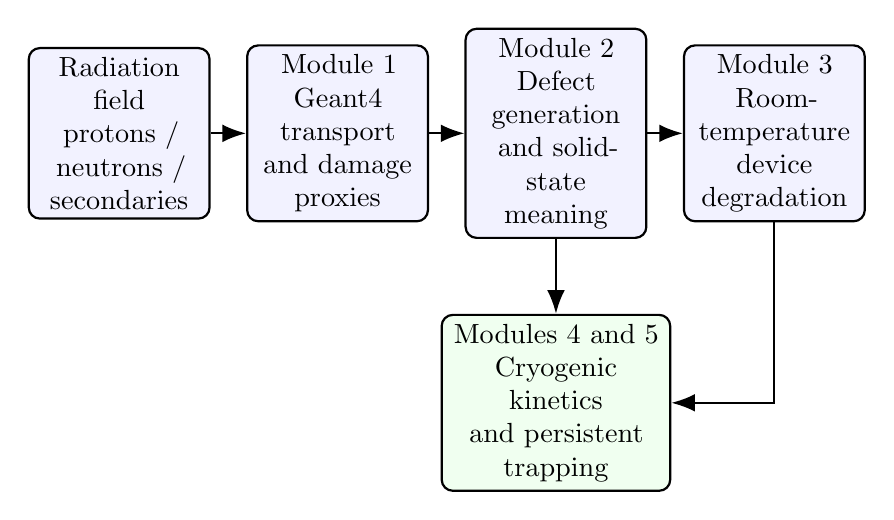
\begin{tikzpicture}[
node distance=0.7cm and 0.45cm,
box/.style={draw, rounded corners=4pt, thick, align=center, minimum height=1.15cm, text width=0.17\textwidth, fill=blue!5},
arrow/.style={-{Latex[length=3mm]}, thick}
]
\node[box] (rad) {Radiation field\\protons / neutrons / secondaries};
\node[box, right=of rad] (g4) {Module 1\\Geant4 transport\\and damage proxies};
\node[box, right=of g4] (def) {Module 2\\Defect generation\\and solid-state meaning};
\node[box, right=of def] (dev) {Module 3\\Room-temperature\\device degradation};
\node[box, below=0.95cm of def, text width=0.22\textwidth, fill=green!6] (cryo) {Modules 4 and 5\\Cryogenic kinetics\\and persistent trapping};

\draw[arrow] (rad) -- (g4);
\draw[arrow] (g4) -- (def);
\draw[arrow] (def) -- (dev);
\draw[arrow] (def) -- (cryo);
\draw[arrow] (dev) |- (cryo);
\end{tikzpicture}
\end{center}

The key structural idea is that Modules 1--3 form the main room-temperature chain, while Modules 4--5 are an extension that asks how the defect landscape changes when the silicon is cooled toward the cryogenic limit.

\section{What each module contributes}
\subsection{Module 1: Geant4 transport and damage proxies}
This module is the front end. It answers: what interactions occur inside silicon before we ever talk about defects? Geant4 provides
\begin{itemize}
    \item event-by-event deposited energy,
    \item depth-dependent deposited energy,
    \item recoil-like ion secondaries as a proxy for strong lattice perturbation.
\end{itemize}

The central caution is that Geant4 does \emph{not} directly give a final, annealed defect chemistry. It gives the collision history from which we construct a physically motivated bridge to defect formation.

\subsection{Module 2: Defect generation and solid-state interpretation}
This module converts transport outputs into a defect-centered picture. The main bridge is a first-order relation such as
\begin{equation}
N_D \propto \Phi
\qquad \text{or} \qquad
N_D(z) \propto D_{\mathrm{proxy}}(z),
\end{equation}
where $N_D$ is defect density, $\Phi$ is fluence, and $D_{\mathrm{proxy}}(z)$ is a damage proxy from Module 1.

Physically, this is the stage where vacancies, interstitials, and defect complexes enter the story. It is where the project moves from radiation transport into solid-state physics.

\subsection{Module 3: Room-temperature device degradation}
This module connects defects to measurable semiconductor degradation. Representative relations are
\begin{equation}
\frac{1}{\taueff} = \frac{1}{\tau_0} + K_\tau N_D,
\end{equation}
\begin{equation}
L = \sqrt{D\,\taueff},
\end{equation}
\begin{equation}
\Delta I = \alpha \Phi V.
\end{equation}
These equations connect defects to lifetime reduction, diffusion-length reduction, and leakage-current increase.

A good analogy is traffic flow in a city. Defects are like intersections blocked by construction. Carriers have a harder time moving efficiently, more of them get delayed or lost, and the overall traffic quality degrades.

\subsection{Module 4: Cryogenic defect kinetics}
This module asks how the \emph{behavior} of existing defects changes with temperature. It focuses on three thermally activated processes:
\begin{equation}
D_{\mathrm{def}}(T) = D_0 \exp\!\left(-\frac{E_m}{\kb T}\right),
\end{equation}
\begin{equation}
e(T) = e_0 \exp\!\left(-\frac{E_a}{\kb T}\right),
\end{equation}
\begin{equation}
R_{\mathrm{ann}}(T) = R_0 \exp\!\left(-\frac{E_{\mathrm{ann}}}{\kb T}\right).
\end{equation}
As temperature drops, migration, emission, and annealing all slow dramatically. The main message is not that defects disappear in the cold. The message is that many of their \emph{kinetics} freeze out.

\subsection{Module 5: Persistent trapping and slow recovery}
This module turns the cryogenic kinetics into one concrete device consequence. A simple recovery model is
\begin{equation}
Q_{\mathrm{trap}}(t,T) = Q_0 \exp\!\left(-\frac{t}{\tau_{\mathrm{rec}}(T)}\right),
\end{equation}
with
\begin{equation}
\tau_{\mathrm{rec}}(T) = \tau_{00} \exp\!\left(\frac{E_r}{\kb T}\right).
\end{equation}
The interpretation is intuitive: at low temperature, the recovery clock can become so slow that the device effectively remembers part of its radiation history over operational timescales.

\section{Development order versus run order}
These two ideas are different, and separating them removes confusion.

\subsection{Development order}
Development order means the order in which the project was architected and expanded:
\begin{enumerate}[label=\arabic*.]
    \item build the room-temperature physics chain,
    \item connect Geant4 outputs to that chain,
    \item add cryogenic defect kinetics,
    \item add persistent trapping as the cryogenic device consequence.
\end{enumerate}
This order is about project design and scope growth.

\subsection{Practical run order}
Practical run order means the easiest order for the user to execute and understand the scripts:
\begin{enumerate}[label=\arabic*.]
    \item run the self-contained room-temperature MATLAB pipeline,
    \item run the cryogenic kinetics extension,
    \item run the persistent trapping extension,
    \item only after Geant4 CSV files exist, run the Geant4-import MATLAB pipeline.
\end{enumerate}
This order is about learning and debugging without being blocked by Geant4 setup.

\section{How the code layers map onto the physics}
\begin{center}
\rowcolors{2}{gray!8}{white}
\begin{tabularx}{\textwidth}{>{\bfseries}p{0.26\textwidth} >{\bfseries}p{0.24\textwidth} Y}
\toprule
Code component & Physics role & Typical use \\
\midrule
Geant4 application & Radiation transport and collision history & Produce damage proxies and spatial interaction data \\
main\_full\_pipeline.m & Core room-temperature degradation model & Learn the main defect-to-device chain without Geant4 input \\
main\_import\_geant4\_pipeline.m & Geant4-coupled degradation model & Map Geant4 output into depth-dependent or fluence-based damage input \\
main\_cryogenic\_extension.m & Cryogenic kinetics model & Study migration, trap emission, and annealing freeze-out \\
main\_persistent\_trapping\_extension.m & Cryogenic device consequence model & Show slow recovery and radiation-history persistence \\
\bottomrule
\end{tabularx}
\end{center}

\section{What the user should remember}
\begin{itemize}
    \item This is one project, not five unrelated documents.
    \item Modules 1--3 form the main radiation-to-device chain.
    \item Modules 4--5 are a cryogenic extension of that same chain.
    \item Development order and run order are different on purpose.
    \item The whole project becomes strongest when discussed as one causal story rather than as isolated equations.
\end{itemize}

\end{document}
